\documentclass[11pt]{article}
\usepackage{amsmath, amssymb, physics, mathtools, bm}
\usepackage{tikz, pgfplots}
\pgfplotsset{compat=1.18}
\usepackage[margin=2.3cm]{geometry}
\usepackage{siunitx, booktabs, hyperref}
\usepackage{braket}

\newcommand{\D}{\mathrm{D}}
\newcommand{\de}{\mathrm{d}}
\newcommand{\pd}[2]{\frac{\partial #1}{\partial #2}}
\newcommand{\pdd}[2]{\frac{\partial^{2} #1}{\partial #2^{2}}}
\newcommand{\Lap}{\nabla^{2}}
\newcommand{\rhat}{\hat{\mathbf{r}}}
\newcommand{\thhat}{\hat{\boldsymbol{\theta}}}
\newcommand{\xhat}{\hat{\mathbf{x}}}
\newcommand{\yhat}{\hat{\mathbf{y}}}
\newcommand{\zhat}{\hat{\mathbf{z}}}

\title{B1 Fluids, 2021 --- Model Solutions}
\author{}
\date{}

\begin{document}
\maketitle

%==============================================================
\section*{Question 1 --- Stokes flow between hinged plates}

\textbf{Problem.} High vs low Re; biharmonic streamfunction; viscous flow between two long, wide plates hinged at $r=0$, opening at constant $\dot\alpha$; verify the quoted $\psi$, find breakdown scales, flux, force scaling, and discuss the scallop theorem.

\subsection*{(a) High vs low Reynolds number}

Re $=UL/\nu$ measures inertia/viscous force ratio.
High Re ($\gg 1$): inertia dominates; viscosity confined to thin boundary layers $\delta\sim L/\sqrt{\mathrm{Re}}$; turbulence; form drag.
Low Re ($\ll 1$): linear Stokes equation $\nabla p=\mu\Lap\vb v$; time-reversible, instantaneous, drag $\propto U$.

Swimming human: $L\sim\SI{1}{m}$, $U\sim\SI{1}{m\,s^{-1}}$, $\nu=\SI{e-6}{m^2 s^{-1}}$.
Plug in numbers:
\[ \mathrm{Re}\sim \frac{(1)(1)}{10^{-6}}. \]
Evaluate:
\[ \mathrm{Re}\sim 10^{6}. \]
\[ \boxed{\;\mathrm{Re}\sim 10^{6}\gg 1:\text{ high-Re regime.}\;} \]

\subsection*{(b) Streamfunction and biharmonic equation}

Polar incompressibility:
\[ \nabla\cdot\vb v = \frac{1}{r}\pd{(rv_r)}{r}+\frac{1}{r}\pd{v_\theta}{\theta}. \]
Substitute $v_r=(1/r)\partial_\theta\psi$, $v_\theta=-\partial_r\psi$:
\[ \nabla\cdot\vb v = \frac{1}{r}\pd{}{r}\!\left(\pd{\psi}{\theta}\right) - \frac{1}{r}\pd{}{\theta}\!\left(\pd{\psi}{r}\right). \]
Equality of mixed partials:
\[ \nabla\cdot\vb v = 0. \]

Vorticity in 2D: $\bm\omega=\omega\zhat$, $\omega=-\Lap\psi$.
At low Re, drop inertia in NS:
\begin{equation}
\nabla p = \mu\Lap\vb v.
\label{eq:stokes}
\end{equation}
Take curl of \eqref{eq:stokes}:
\[ \nabla\times\nabla p = 0 = \mu\Lap(\nabla\times\vb v). \]
Use $\nabla\times\vb v = \omega\zhat$ in 2D:
\[ 0 = \mu\Lap\bm\omega. \]
Substitute $\omega=-\Lap\psi$:
\begin{equation}
\boxed{\;\Lap^{2}\psi = \nabla^{4}\psi = 0.\;}
\label{eq:biharm}
\end{equation}

\subsection*{(c) Boundary conditions and verification}

\paragraph{BCs.} No-slip on the fixed plate ($\theta=0$):
\[ v_r(r,0)=0,\quad v_\theta(r,0)=0\;\Longrightarrow\; \pd{\psi}{\theta}\bigg|_{0}=0,\quad \pd{\psi}{r}\bigg|_{0}=0. \]
Rigid rotation of upper plate ($\theta=\alpha$): $\vb v_{\rm plate}=r\dot\alpha\thhat$:
\[ v_r(r,\alpha)=0,\quad v_\theta(r,\alpha)=r\dot\alpha\;\Longrightarrow\; \pd{\psi}{\theta}\bigg|_{\alpha}=0,\quad \pd{\psi}{r}\bigg|_{\alpha}=-r\dot\alpha. \]

\paragraph{Ansatz.} BC linear in $r$ forces $n=2$:
\[ \psi(r,\theta) = r^{2}f(\theta),\qquad f(\theta) = A\cos 2\theta+B\sin 2\theta+C\theta\cos 2\theta+D\theta\sin 2\theta. \]
Reduce BCs by dividing $r^{2}$ and $2r$:
\[ f(0)=0,\quad f'(0)=0,\quad f(\alpha)=-\tfrac12\dot\alpha,\quad f'(\alpha)=0. \]
Apply $f(0)=0$:
\[ A=0. \]
Differentiate $f$:
\[ f'(\theta)=-2A\sin 2\theta+2B\cos 2\theta+C(\cos 2\theta-2\theta\sin 2\theta)+D(\sin 2\theta+2\theta\cos 2\theta). \]
Apply $f'(0)=0$:
\[ 2B+C=0\;\Longrightarrow\; C=-2B. \]
Reduced $f$:
\[ f(\theta)=B\sin 2\theta-2B\theta\cos 2\theta+D\theta\sin 2\theta. \]
Reduced $f'$:
\[ f'(\theta) = 4B\theta\sin 2\theta + D(\sin 2\theta+2\theta\cos 2\theta). \]
Write $s=\sin 2\alpha$, $c=\cos 2\alpha$. The two upper-plate conditions become
\[ 4B\alpha s + D(s+2\alpha c) = 0, \]
\[ B(s-2\alpha c) + D\alpha s = -\tfrac12\dot\alpha. \]
Determinant:
\[ \Delta = 4\alpha^{2}s^{2} - (s+2\alpha c)(s-2\alpha c). \]
Cramer for $B$:
\[ B = \frac{\dot\alpha(s+2\alpha c)}{2\Delta}. \]
Cramer for $D$:
\[ D = -\frac{2\alpha s\,\dot\alpha}{\Delta}. \]
Insert $B,D$ into reduced $f$:
\[ f(\theta) = \frac{\dot\alpha(s+2\alpha c)}{2\Delta}(\sin 2\theta - 2\theta\cos 2\theta) - \frac{2\alpha s\,\dot\alpha}{\Delta}\,\theta\sin 2\theta. \]
Factor $\dot\alpha/(2\Delta)$:
\[ f(\theta) = \frac{\dot\alpha}{2\Delta}\bigl[(s+2\alpha c)(\sin 2\theta - 2\theta\cos 2\theta) - 4\alpha s\,\theta\sin 2\theta\bigr]. \]
Rewrite with overall minus sign to match quoted form:
\[ f(\theta) = -\frac{\dot\alpha}{2\Delta}\bigl[4\alpha s\,\theta\sin 2\theta - (s+2\alpha c)(\sin 2\theta - 2\theta\cos 2\theta)\bigr]. \]
Multiply by $r^{2}$:
\begin{equation}
\boxed{\;\psi = -\frac{\dot\alpha\,r^{2}}{2}\,\frac{(4\alpha\sin 2\alpha)(\theta\sin 2\theta)-(\sin 2\alpha+2\alpha\cos 2\alpha)(\sin 2\theta-2\theta\cos 2\theta)}{4\alpha^{2}\sin^{2}2\alpha-(\sin 2\alpha+2\alpha\cos 2\alpha)(\sin 2\alpha-2\alpha\cos 2\alpha)}\;}
\label{eq:psi-quoted}
\end{equation}
which matches the quoted formula with $\Omega=\dot\alpha$.

\paragraph{Breakdown scales.} Local Reynolds number with $U\sim r\dot\alpha$:
\[ \mathrm{Re}_{\rm loc} = \frac{Ur}{\nu} \sim \frac{r^{2}\dot\alpha}{\nu}. \]
Stokes validity demands:
\[ \frac{r^{2}\dot\alpha}{\nu} \lesssim 1. \]
Solve for $r$:
\[ l_1 = \sqrt{\nu/\dot\alpha}. \]
End-effects of finite plate length set a second scale:
\[ l_2 = L. \]
\[ \boxed{\;l_1=\sqrt{\nu/\dot\alpha},\qquad l_2 = L.\;} \]

\subsection*{(d) Volume flux through cylinder of radius $r$}

Flux per unit length:
\[ Q(r) = \int_{0}^{\alpha} v_r\,r\,\de\theta. \]
Substitute $v_r = (1/r)\partial_\theta\psi$:
\[ Q(r) = \int_{0}^{\alpha}\pd{\psi}{\theta}\,\de\theta. \]
Evaluate antiderivative:
\[ Q(r) = \psi(r,\alpha)-\psi(r,0). \]
Use $\psi = r^{2}f(\theta)$ with $f(0)=0$, $f(\alpha)=-\tfrac12\dot\alpha$:
\begin{equation}
\boxed{\;Q(r) = -\tfrac12\dot\alpha\,r^{2}.\;}
\label{eq:Q}
\end{equation}
Geometric meaning: rate of area swept inside radius $r$ as $\alpha$ grows is $\tfrac12 r^{2}\dot\alpha$, so fluid is drawn in across the cylinder at exactly that rate (mass conservation).

\subsection*{(e) Free hinge: pressure, force, scallop theorem}

\paragraph{Pressure.} With $\psi$ known, $\vb v$ is known; integrate Stokes \eqref{eq:stokes}:
\[ \nabla p = \mu\Lap\vb v = -\mu\,\nabla\times(\omega\zhat). \]
Line-integrate from a reference point; fix the constant by matching ambient pressure at $r=L$.

\paragraph{Force scaling.} Stokes flow is linear in boundary velocity, so $p\sim\mu\dot\alpha$ (independent of $r$ to leading order); plate length $L$:
\[ F\sim p\cdot L. \]
\[ \boxed{\;F\propto \mu L\dot\alpha.\;} \]

\paragraph{Scallop theorem.} Periodic $\alpha(t)$, period $T$. Net impulse:
\[ \mathcal I = \oint F\,\de t. \]
Substitute $F\propto \mu L\dot\alpha$:
\[ \mathcal I \propto \mu L\oint\dot\alpha\,\de t. \]
Integrate $\dot\alpha$:
\[ \mathcal I \propto \mu L[\alpha(T)-\alpha(0)]. \]
Apply periodicity $\alpha(T)=\alpha(0)$:
\[ \mathcal I = 0. \]
A reciprocal one-DOF gait produces no net displacement (Purcell 1977). Cyclic opening and closing of a hinged scallop cannot generate propulsion at low Re; non-reciprocal gaits (e.g.\ rotating helical flagella) are required.

%==============================================================
\section*{Question 2 --- Sound waves in a moving medium}

\textbf{Problem.} Mechanism of sound; convected wave equation in a uniform stream $U_0\xhat$; dispersion; observers up- and downstream; supersonic and transonic cases.

\subsection*{(a) Mechanism of sound propagation}

A local compression raises $p$ above ambient. Pressure gradient $-\partial_x p$ accelerates neighbouring fluid outward (Newton: $\rho_0\partial_t v=-\partial_x p$). Mass piles into next layer; that layer compresses; the bump translates. Speed: inertia/compressibility balance $c_0=\sqrt{\partial p/\partial\rho|_{\rho_0}}$. Pulse splits into left- and right-going branches (d'Alembert).

\begin{center}
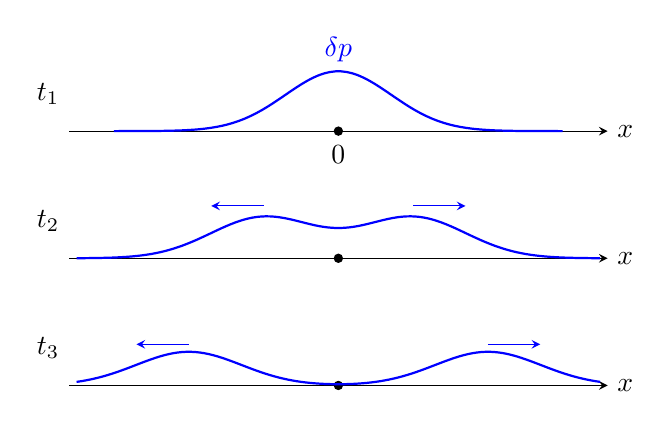
\begin{tikzpicture}[scale=0.95,>=stealth]
  \draw[->] (-3.6,0) -- (3.6,0) node[right]{$x$};
  \node[circle,fill,inner sep=1.2pt,label=below:{$0$}] at (0,0) {};
  \draw[thick,blue] plot[domain=-3:3,samples=80] (\x, {0.8*exp(-(\x)^2)});
  \node[blue,above] at (0,0.8) {$\delta p$};
  \node[left] at (-3.6,0.5) {$t_1$};

  \begin{scope}[yshift=-1.7cm]
  \draw[->] (-3.6,0) -- (3.6,0) node[right]{$x$};
  \node[circle,fill,inner sep=1.2pt] at (0,0) {};
  \draw[thick,blue] plot[domain=-3.5:3.5,samples=120] (\x, {0.55*exp(-(\x-1.0)^2)+0.55*exp(-(\x+1.0)^2)});
  \draw[->,blue] (-1,0.7) -- (-1.7,0.7);
  \draw[->,blue] ( 1,0.7) -- ( 1.7,0.7);
  \node[left] at (-3.6,0.5) {$t_2$};
  \end{scope}

  \begin{scope}[yshift=-3.4cm]
  \draw[->] (-3.6,0) -- (3.6,0) node[right]{$x$};
  \node[circle,fill,inner sep=1.2pt] at (0,0) {};
  \draw[thick,blue] plot[domain=-3.5:3.5,samples=120] (\x, {0.45*exp(-(\x-2.0)^2)+0.45*exp(-(\x+2.0)^2)});
  \draw[->,blue] (-2,0.55) -- (-2.7,0.55);
  \draw[->,blue] ( 2,0.55) -- ( 2.7,0.55);
  \node[left] at (-3.6,0.5) {$t_3$};
  \end{scope}
\end{tikzpicture}
\end{center}

\subsection*{(b) Linearisation: convected wave equation}

Write $\rho=\rho_0+\rho_1$, $p=p_0+p_1$, $v=U_0+v_1$.

Continuity:
\[ \pd{\rho}{t}+\nabla\cdot(\rho\vb v)=0. \]
Substitute $\rho=\rho_0+\rho_1$, $v=U_0+v_1$:
\[ \pd{\rho_1}{t} + \pd{}{x}[(\rho_0+\rho_1)(U_0+v_1)] = 0. \]
Expand the product:
\[ \pd{\rho_1}{t} + \pd{}{x}[\rho_0 U_0 + \rho_0 v_1 + U_0\rho_1 + \rho_1 v_1] = 0. \]
Drop the constant $\rho_0 U_0$ and the quadratic $\rho_1 v_1$:
\begin{equation}
\D\rho_1 + \rho_0\pd{v_1}{x}=0,\qquad \D\equiv\pd{}{t}+U_0\pd{}{x}.
\label{eq:cont}
\end{equation}
1-D inviscid Euler:
\[ \pd{v}{t} + v\pd{v}{x} + \frac{1}{\rho}\pd{p}{x} = 0. \]
Substitute background plus perturbation:
\[ \pd{v_1}{t} + (U_0+v_1)\pd{v_1}{x} + \frac{1}{\rho_0+\rho_1}\pd{p_1}{x} = 0. \]
Drop quadratic $v_1\partial_x v_1$ and expand $1/(\rho_0+\rho_1)\approx 1/\rho_0$:
\begin{equation}
\D v_1 = -\frac{1}{\rho_0}\pd{p_1}{x}.
\label{eq:mom}
\end{equation}
Polytropic state $p=p_0(\rho/\rho_0)^\gamma$; differentiate at $\rho=\rho_0$:
\[ \dv{p}{\rho}\bigg|_{\rho_0} = \gamma p_0/\rho_0 \equiv c_0^{2}. \]
Linearise:
\begin{equation}
p_1 = c_0^{2}\rho_1.
\label{eq:eos}
\end{equation}
Apply $\D$ to \eqref{eq:cont}:
\[ \D^{2}\rho_1 + \rho_0\,\D\!\left(\pd{v_1}{x}\right) = 0. \]
Commute $\D$ and $\partial_x$:
\[ \D^{2}\rho_1 + \rho_0\pd{(\D v_1)}{x} = 0. \]
Substitute \eqref{eq:mom}:
\[ \D^{2}\rho_1 + \pd{}{x}\!\left(-\pd{p_1}{x}\right) = 0. \]
Simplify:
\[ \D^{2}\rho_1 = \pdd{p_1}{x}. \]
Substitute \eqref{eq:eos}:
\[ \D^{2}\rho_1 = c_0^{2}\pdd{\rho_1}{x}. \]
Hence
\begin{equation}
\boxed{\;\!\!\left(\pd{}{t}+U_0\pd{}{x}\right)\!\!\left(\pd{}{t}+U_0\pd{}{x}\right)\rho_1 = c_0^{2}\pdd{\rho_1}{x}.\;}
\label{eq:wave}
\end{equation}

\subsection*{(c) Dispersion and snapshot at $U_0=0$}

Plane wave $\rho_1=\rho_0 A\,e^{i(kx-\omega t)}$ in \eqref{eq:wave}:
\[ (-i\omega+iU_0 k)^{2}\rho_1 = -c_0^{2}k^{2}\rho_1. \]
Cancel $\rho_1$:
\[ (-i\omega+iU_0 k)^{2} = -c_0^{2}k^{2}. \]
Take the square root:
\[ -i(\omega-U_0 k) = \pm ic_0 k. \]
Divide by $-i$:
\[ \omega-U_0 k = \pm c_0 k. \]
\begin{equation}
\boxed{\;\omega = (U_0\pm c_0)k.\;}
\label{eq:disp}
\end{equation}
Invert for $k$ at fixed $\omega$:
\[ k_\pm = \frac{\omega}{U_0\pm c_0}. \]

\paragraph{Snapshot $U_0=0$, $\omega t=2n\pi$.} Outgoing-wave d'Alembert solution from source at $x=0$:
\[ \rho_1 = \rho_0 A\cos\!\bigl[\omega t - k_0|x|\bigr],\qquad k_0=\omega/c_0. \]
Set $\omega t=2n\pi$ and use even cosine:
\[ \rho_1 = \rho_0 A\cos(k_0|x|). \]
Apply \eqref{eq:eos}:
\[ p_1 = c_0^{2}\rho_0 A\cos(k_0|x|). \]
Take right-going wave for $x>0$:
\[ p_1 = c_0^{2}\rho_0 A\cos(\omega t - k_0 x). \]
Differentiate in $x$:
\[ \pd{p_1}{x} = c_0^{2}\rho_0 A k_0\sin(\omega t - k_0 x). \]
Use \eqref{eq:mom} with $U_0=0$:
\[ \rho_0\pd{v_1}{t} = -\pd{p_1}{x} = -c_0^{2}\rho_0 A k_0\sin(\omega t - k_0 x). \]
Integrate in $t$ using $k_0=\omega/c_0$:
\[ v_1 = c_0 A\cos(\omega t - k_0 x). \]
Set $\omega t=2n\pi$:
\[ v_1(x>0) = c_0 A\cos(k_0 x). \]
Left-going wave for $x<0$ gives the opposite sign:
\[ v_1 = \mathrm{sgn}(x)\,c_0 A\cos(k_0|x|). \]
$\rho_1, p_1$ even in $x$; $v_1$ odd (radiation away from source).

\begin{center}
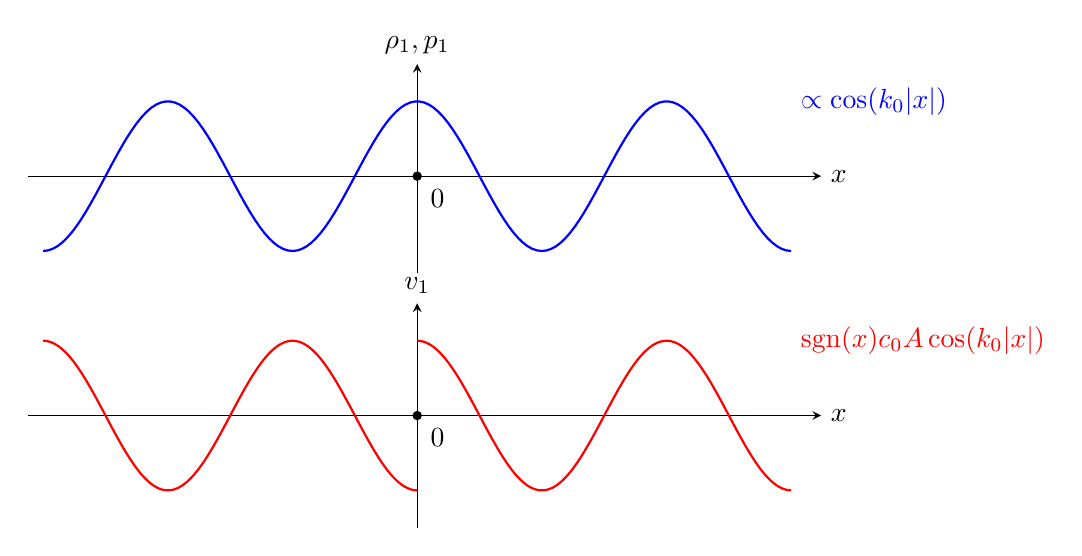
\begin{tikzpicture}[scale=0.95,>=stealth]
  \draw[->] (-5.2,0) -- (5.4,0) node[right]{$x$};
  \draw[->] (0,-1.3) -- (0,1.5) node[above]{$\rho_1, p_1$};
  \node[circle,fill,inner sep=1.2pt,label=below right:{$0$}] at (0,0) {};
  \draw[thick,blue] plot[domain=-5:5,samples=160] (\x, {1.0*cos(180*\x*0.6)});
  \node[blue,right] at (5,1.0) {$\propto\cos(k_0|x|)$};

  \begin{scope}[yshift=-3.2cm]
  \draw[->] (-5.2,0) -- (5.4,0) node[right]{$x$};
  \draw[->] (0,-1.5) -- (0,1.5) node[above]{$v_1$};
  \node[circle,fill,inner sep=1.2pt,label=below right:{$0$}] at (0,0) {};
  \draw[thick,red] plot[domain=0.001:5,samples=160] (\x, {1.0*cos(180*\x*0.6)});
  \draw[thick,red] plot[domain=-5:-0.001,samples=160] (\x, {-1.0*cos(180*\x*0.6)});
  \node[red,right] at (5,1.0) {$\mathrm{sgn}(x)c_0 A\cos(k_0|x|)$};
  \end{scope}
\end{tikzpicture}
\end{center}

\subsection*{(d) Two observers; supersonic; $U_0\to c_0$}

Lab-frame wavelengths from $k_\pm$:
\[ \lambda_\pm = \frac{2\pi}{|k_\pm|} = \frac{2\pi|U_0\pm c_0|}{\omega}. \]

\paragraph{Subsonic $U_0<c_0$.} Both observers see frequency $\omega$ (steady forcing in lab frame). Downstream ($x=+L$): wavelength
\[ \lambda_+ = \frac{2\pi(U_0+c_0)}{\omega}\quad\text{(stretched)}. \]
Upstream ($x=-L$): wavelength
\[ |\lambda_-| = \frac{2\pi(c_0-U_0)}{\omega}\quad\text{(compressed)}. \]
Wavecounts in window of length $l$: $N_\pm = l/|\lambda_\pm|$:
\[ \frac{N_-}{N_+} = \frac{|\lambda_+|}{|\lambda_-|} = \frac{U_0+c_0}{c_0-U_0}. \]

\paragraph{Supersonic $U_0>c_0$.} Both $k_\pm>0$; both branches advected downstream. At $x=+L$ a beat pattern of two waves with $k_\pm=\omega/(U_0\pm c_0)$. At $x=-L$: nothing — no characteristic reaches $x=-L$ from $x=0$.

\paragraph{Limit $U_0\to c_0^{-}$.} $\lambda_-\to 0$, lab phase speed $c_0-U_0\to 0$; upstream wave is frozen and energy density diverges under finite forcing. Linear theory breaks down: nonlinear steepening (shock) and dissipation must be reintroduced — the transonic singularity.

%==============================================================
\section*{Question 3 --- Lubrication theory for a sessile drop}

\textbf{Problem.} Thin axisymmetric drop, density $\rho$, viscosity $\mu$, surface tension $\gamma$, gravity $g$. Justify lubrication NS, derive $p(r,z,t)$ and the parabolic $\vb v$. Volume flux gives the thin-film PDE. Steady state with $\kappa\approx-\partial_r^{2}h$, contact angle $\theta_c$, regularity at $r=0$, volume $V$.

\subsection*{(a) Lubrication, pressure, horizontal velocity}

Let $H,L$ be vertical/horizontal scales, $\epsilon\equiv H/L\ll 1$. From continuity $U/L\sim W/H$:
\[ W\sim\epsilon U\ll U. \]
Reduced Reynolds (inertia/viscous):
\[ \frac{\rho U^{2}/L}{\mu U/H^{2}} = \mathrm{Re}\,\epsilon^{2}\ll 1. \]
Compare streamwise to vertical viscous derivatives:
\[ \frac{\partial_x^{2}\vb v}{\partial_z^{2}\vb v} \sim \frac{H^{2}}{L^{2}} = \epsilon^{2}\ll 1. \]
Drop inertia and streamwise viscous term in NS:
\begin{equation}
\boxed{\;0\approx \mu\pdd{\vb v}{z} - \nabla p - \rho g\zhat.\;}
\label{eq:lub}
\end{equation}

\paragraph{Pressure.} Take $z$-component of \eqref{eq:lub}:
\[ \pd{p}{z} = -\rho g. \]
Integrate in $z$:
\[ p(r,z,t) = -\rho g z + f(r,t). \]
Apply Young--Laplace $p|_-^+ = p_0 - p(r,h) = -\gamma\kappa$, i.e.\ $p(r,h) = p_0+\gamma\kappa$:
\[ -\rho g h + f = p_0 + \gamma\kappa. \]
Solve for $f$:
\[ f = p_0 + \rho g h + \gamma\kappa. \]
Hence
\begin{equation}
\boxed{\;p(r,z,t) = p_0 + \rho g(h-z) + \gamma\kappa(r,t).\;}
\label{eq:p}
\end{equation}

\paragraph{Horizontal velocity.} Take radial component of \eqref{eq:lub}:
\[ \mu\pdd{v_r}{z} = \pd{p}{r}. \]
Differentiate \eqref{eq:p} in $r$:
\[ \pd{p}{r} = \rho g\pd{h}{r} + \gamma\pd{\kappa}{r}. \]
Abbreviate the driving term:
\[ G(r,t) \equiv \rho g\,\pd{h}{r} + \gamma\pd{\kappa}{r}. \]
Integrate $\mu\partial_z^{2}v_r = G$ once with $\partial_z v_r|_{z=h}=0$ (no surface stress):
\[ \mu\pd{v_r}{z} = G(z-h). \]
Integrate again with $v_r(0)=0$ (no-slip on $z=0$):
\[ \mu v_r = G\!\left(\tfrac12 z^{2} - hz\right). \]
Factor $z/2$:
\[ \mu v_r = \tfrac12 G\,z(z-2h). \]
Vector form:
\begin{equation}
\boxed{\;\vb v\approx\!\left[\rho g\pd{h}{r} + \gamma\pd{\kappa}{r}\right]\!\frac{z(z-2h)}{2\mu}\,\rhat.\;}
\label{eq:v}
\end{equation}

\subsection*{(b) Volume flux and the thin-film equation}

Flux through cylinder of radius $r$:
\[ Q(r,t) = 2\pi r\int_{0}^{h}v_r\,\de z. \]
Substitute \eqref{eq:v}:
\[ Q = \frac{2\pi r}{2\mu}\!\left(\rho g\pd{h}{r}+\gamma\pd{\kappa}{r}\right)\!\int_{0}^{h}z(z-2h)\,\de z. \]
Evaluate the inner integral:
\[ \int_{0}^{h}z(z-2h)\,\de z = \tfrac13 h^{3} - h^{3}. \]
Combine:
\[ \int_{0}^{h}z(z-2h)\,\de z = -\tfrac23 h^{3}. \]
Substitute:
\[ Q(r,t) = -\frac{2\pi r\,h^{3}}{3\mu}\!\left(\rho g\pd{h}{r}+\gamma\pd{\kappa}{r}\right). \]
Annular mass balance for $r\le r'\le r+\de r$:
\[ \pd{}{t}(2\pi r\,h\,\de r) = -\pd{Q}{r}\de r. \]
Cancel $\de r$:
\[ 2\pi r\,\pd{h}{t} = -\pd{Q}{r}. \]
Divide by $2\pi r$:
\[ \pd{h}{t} = -\frac{1}{2\pi r}\pd{Q}{r}. \]
Substitute $Q$ and rearrange:
\begin{equation}
\boxed{\;\pd{h}{t} = \frac{1}{r}\pd{}{r}\!\left[r\frac{h^{3}}{3\mu}\!\left(\rho g\pd{h}{r}+\gamma\pd{\kappa}{r}\right)\right].\;}
\label{eq:thinfilm}
\end{equation}

\subsection*{(c) Steady drop shape}

Steady $\partial_t h=0$ implies $Q$ independent of $r$. Boundary $h(R)=0$ forces $Q\equiv 0$. With $h>0$ the bracket vanishes:
\[ \rho g\pd{h}{r} + \gamma\pd{\kappa}{r} = 0. \]
Integrate in $r$:
\[ \rho g\,h + \gamma\kappa = K\quad\text{(const)}. \]
Substitute $\kappa\approx -\partial_r^{2}h$:
\[ \rho g\,h - \gamma\pdd{h}{r} = K. \]
Rearrange:
\[ \gamma\pdd{h}{r} = \rho g\,h - K. \]
Define capillary length:
\[ \boxed{\;l\equiv\sqrt{\gamma/(\rho g)}.\;} \]
Divide by $\gamma$:
\[ \pdd{h}{r} - \frac{1}{l^{2}}h = -\frac{K}{\gamma}. \]
General solution: homogeneous $\cosh$, $\sinh$ plus particular $h_0 = Kl^{2}/\gamma$. Regularity at $r=0$ ($\partial_r h\to 0$) kills the $\sinh$:
\[ h(r) = A_1\cosh(r/l) + h_0,\qquad h_0\equiv Kl^{2}/\gamma. \]
Apply $h(R)=0$:
\[ A_1\cosh(R/l) + h_0 = 0. \]
Solve for $h_0$:
\[ h_0 = -A_1\cosh(R/l). \]
Substitute:
\[ h(r) = A_1\cosh(r/l) - A_1\cosh(R/l). \]
Factor $-A_1$:
\[ h(r) = -A_1[\cosh(R/l) - \cosh(r/l)]. \]
Set $\alpha\equiv -A_1/l>0$:
\begin{equation}
\boxed{\;h(r) = \alpha l\,[\cosh(R/l) - \cosh(r/l)].\;}
\label{eq:h}
\end{equation}
Differentiate $h$:
\[ \pd{h}{r} = -\alpha\sinh(r/l). \]
Apply contact-angle condition $\partial_r h(R)=-\tan\theta_c$:
\[ -\alpha\sinh(R/l) = -\tan\theta_c. \]
Solve for $\alpha$:
\[ \boxed{\;\alpha = \frac{\tan\theta_c}{\sinh(R/l)}.\;} \]
Volume:
\[ V = \int_{0}^{R}2\pi r\,h(r)\,\de r. \]
Substitute \eqref{eq:h}:
\[ V = 2\pi\alpha l\int_{0}^{R}[\cosh(R/l)-\cosh(r/l)]\,r\,\de r. \]
Change variable $\xi=r/l$, $\de r = l\,\de\xi$, $r=l\xi$:
\[ V = 2\pi\alpha l^{3}\int_{0}^{R/l}[\cosh(R/l)-\cosh\xi]\,\xi\,\de\xi. \]
Divide by $V$:
\begin{equation}
\boxed{\;1 = \frac{2\pi l^{3}\alpha}{V}\int_{0}^{R/l}[\cosh(R/l)-\cosh\xi]\,\xi\,\de\xi.\;}
\label{eq:R}
\end{equation}

\paragraph{Force balances.}
Bulk: $\rho g h$ (gravity hydrostatic) vs $-\gamma\partial_r^{2}h$ (capillary Laplace pressure); crossover at the capillary length $l$. $R\ll l$: surface tension dominates, drop is a spherical cap. $R\gg l$: gravity dominates, drop is a flat puddle of thickness $\sim 2l\sin(\theta_c/2)$.
Edge: Young's equation $\gamma_{SV}=\gamma_{SL}+\gamma\cos\theta_c$ fixes $\theta_c$, hence $\alpha$.
Global: \eqref{eq:R} ties $R$ to $V$.

%==============================================================
\section*{Question 4 --- Complex potential and Joukowski mapping}

\textbf{Problem.} Why simple shear has no $w(z)$. Streamfunctions of $w=\beta z^{2}$ and $w=\beta z^{2}e^{i\alpha}$; dyed disc area. Cylinder of radius $a$ in the second flow: find $w=Az^{2}+B/z^{2}$, surface speed, net force. Joukowski map to ellipse: $W(Z)$ and stagnation points.

\subsection*{(a) Why simple shear has no $w(z)$}

$\vb v=(\beta y,0)$. Compute divergence:
\[ \nabla\cdot\vb v = \partial_x(\beta y)+\partial_y(0) = 0. \]
Compute curl:
\[ (\nabla\times\vb v)_z = \partial_x v_y - \partial_y v_x = -\beta. \]
$w(z)=\phi+i\psi$ requires $\vb v=\nabla\phi$ (irrotational) \emph{and} $\nabla\cdot\vb v=0$. Simple shear has uniform vorticity $-\beta\ne 0$, so no $\phi$ exists, hence no $w(z)$.

\subsection*{(b) Streamfunctions and the dyed disc}

\paragraph{(i) $w=\beta z^{2}$.} Substitute $z=x+iy$:
\[ w = \beta(x+iy)^{2}. \]
Expand the square:
\[ w = \beta(x^{2}-y^{2}) + 2i\beta xy. \]
Read off real and imaginary parts:
\[ \boxed{\;\phi=\beta(x^{2}-y^{2}),\qquad \psi=2\beta xy.\;} \]
Streamlines: $xy=$ const (rectangular hyperbolae); axes are $\psi=0$. Pure straining flow with stagnation at origin, principal axes along $x$ and $y$.

\paragraph{(ii) $w=\beta z^{2}e^{i\alpha}$.} Set $z=re^{i\theta}$:
\[ w = \beta r^{2}e^{2i\theta}e^{i\alpha} = \beta r^{2}e^{i(2\theta+\alpha)}. \]
Take imaginary part:
\[ \boxed{\;\psi = \beta r^{2}\sin(2\theta+\alpha).\;} \]
Streamlines are the same hyperbolae rotated by $-\alpha/2$.

\begin{center}
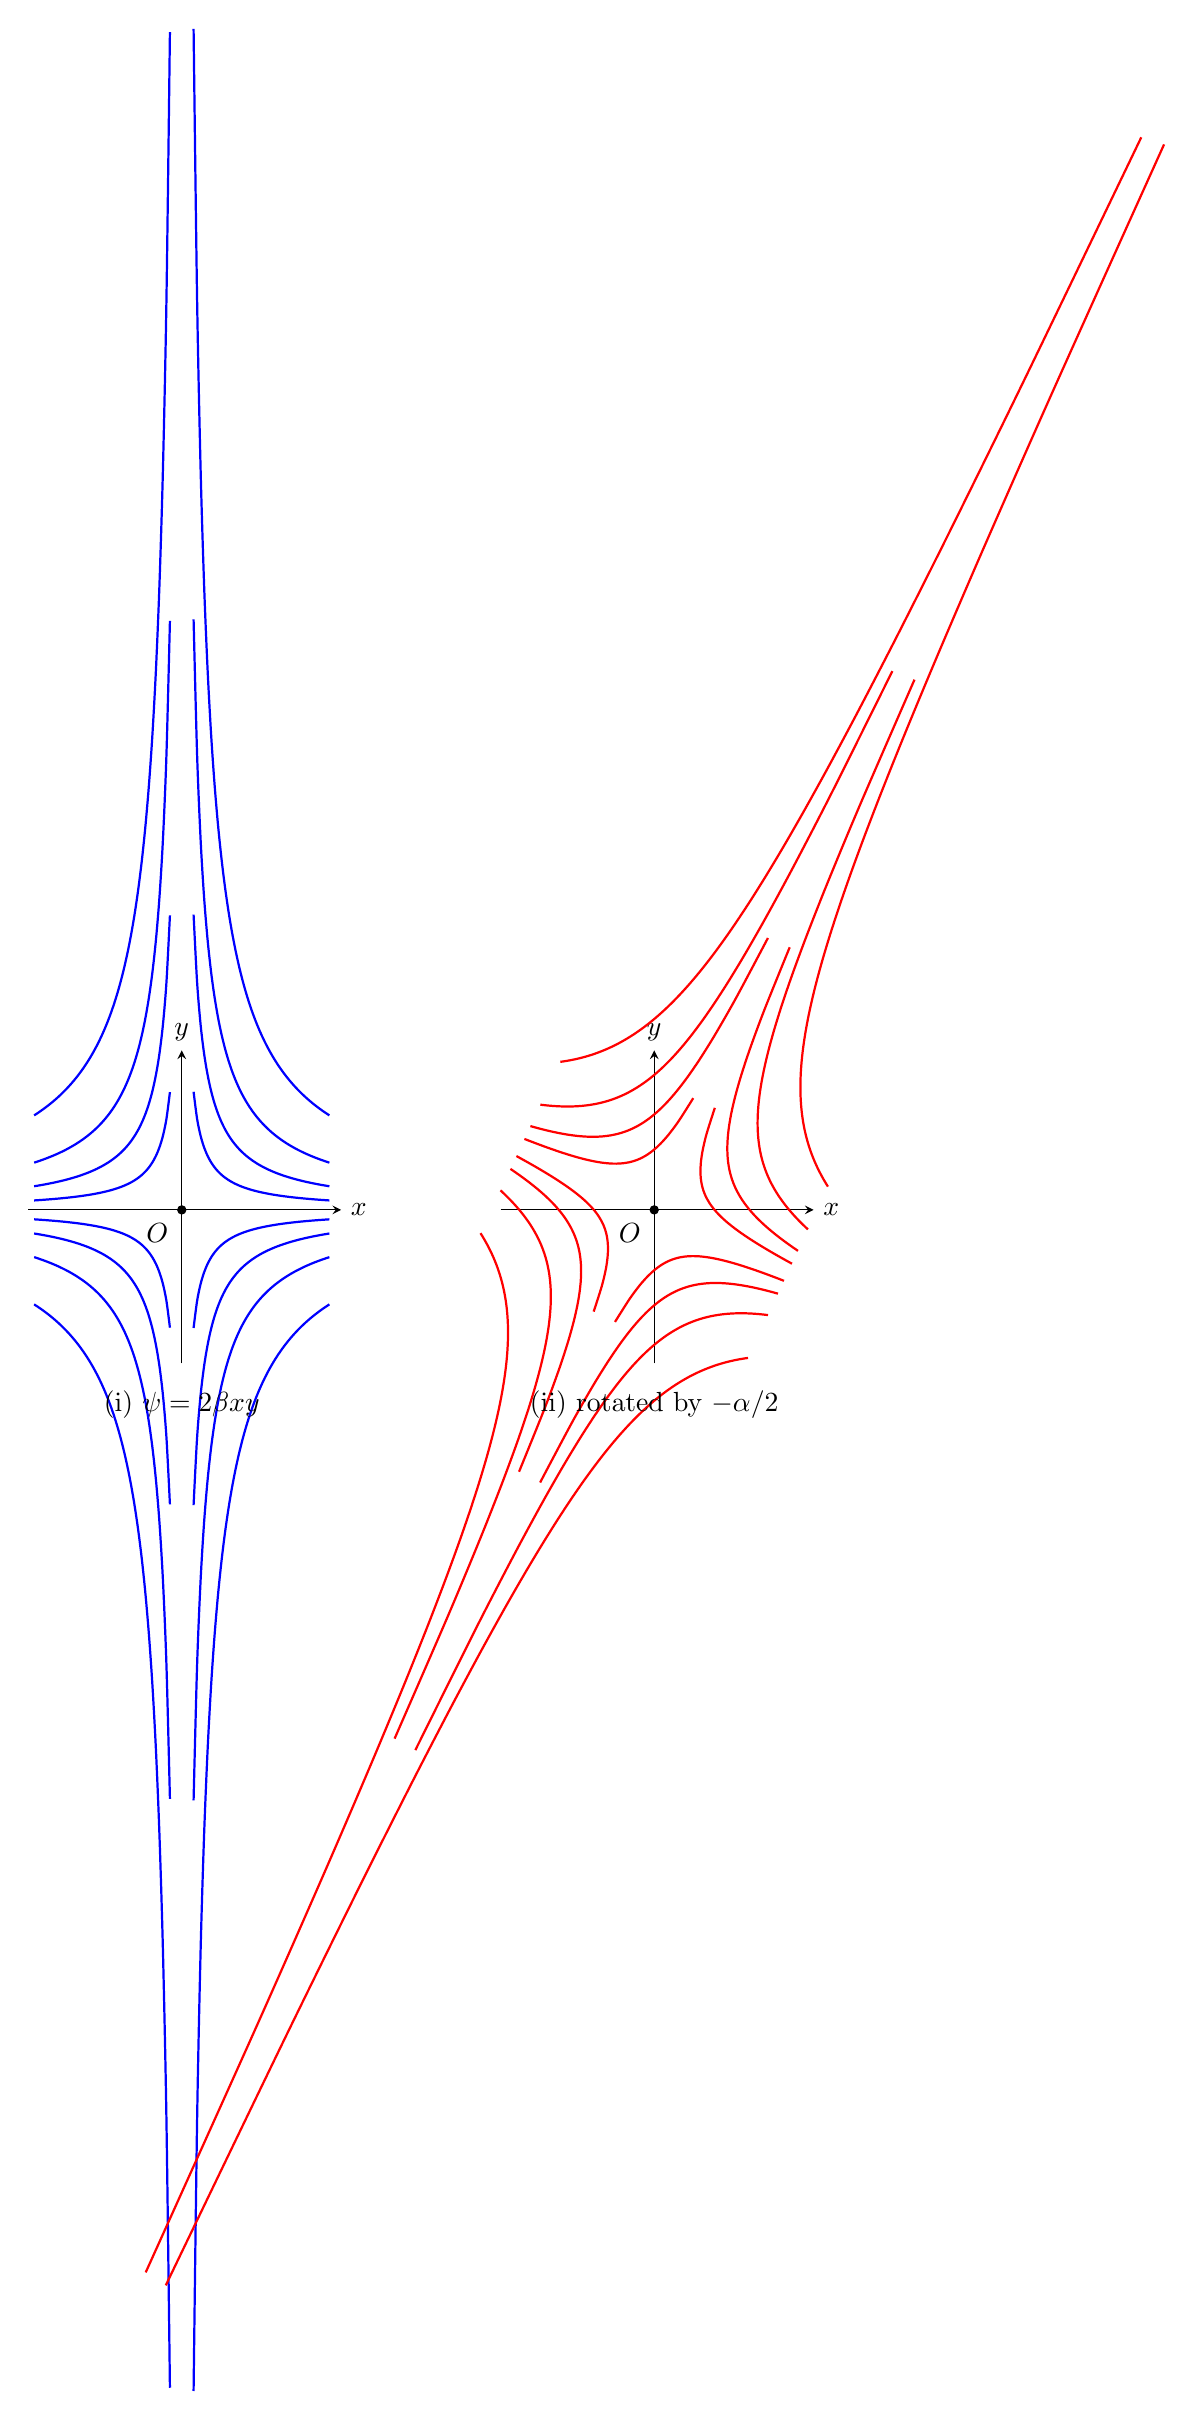
\begin{tikzpicture}[scale=0.75,>=stealth]
  \begin{scope}
  \draw[->] (-2.6,0)--(2.7,0) node[right]{$x$};
  \draw[->] (0,-2.6)--(0,2.7) node[above]{$y$};
  \node[circle,fill,inner sep=1.2pt,label=below left:{$O$}] at (0,0) {};
  \foreach \c in {0.4,1,2,4}{
    \draw[blue,thick,domain=0.2:2.5,smooth,samples=40] plot (\x,{\c/\x});
    \draw[blue,thick,domain=-2.5:-0.2,smooth,samples=40] plot (\x,{\c/\x});
    \draw[blue,thick,domain=0.2:2.5,smooth,samples=40] plot (\x,{-\c/\x});
    \draw[blue,thick,domain=-2.5:-0.2,smooth,samples=40] plot (\x,{-\c/\x});
  }
  \node[below] at (0,-2.9) {(i) $\psi=2\beta xy$};
  \end{scope}
  \begin{scope}[xshift=8cm]
  \draw[->] (-2.6,0)--(2.7,0) node[right]{$x$};
  \draw[->] (0,-2.6)--(0,2.7) node[above]{$y$};
  \node[circle,fill,inner sep=1.2pt,label=below left:{$O$}] at (0,0) {};
  \begin{scope}[rotate=-25]
    \foreach \c in {0.4,1,2,4}{
      \draw[red,thick,domain=0.2:2.5,smooth,samples=40] plot (\x,{\c/\x});
      \draw[red,thick,domain=-2.5:-0.2,smooth,samples=40] plot (\x,{\c/\x});
      \draw[red,thick,domain=0.2:2.5,smooth,samples=40] plot (\x,{-\c/\x});
      \draw[red,thick,domain=-2.5:-0.2,smooth,samples=40] plot (\x,{-\c/\x});
    }
  \end{scope}
  \node[below] at (0,-2.9) {(ii) rotated by $-\alpha/2$};
  \end{scope}
\end{tikzpicture}
\end{center}

\paragraph{Dyed disc area.} 2D incompressible flow conserves material area:
\[ \boxed{\;\text{Area}(t) = \pi R^{2}\;\text{for all }t.\;} \]
The disc deforms into an ellipse: stretches by $e^{2\beta t}$ along the extensional axis, compresses by $e^{-2\beta t}$ along the orthogonal axis. Product unity.

\subsection*{(c) Cylinder in the strain field}

\paragraph{Find $A,B$.} Far-field matching $w\sim\beta z^{2}e^{i\alpha}$ fixes
\[ A = \beta e^{i\alpha}. \]
Evaluate $w$ on $z=ae^{i\theta}$:
\[ w = Aa^{2}e^{2i\theta} + \frac{B}{a^{2}}e^{-2i\theta}. \]
Impermeability requires $\Im w=$ const on $|z|=a$ for all $\theta$. Write $A=\beta(\cos\alpha+i\sin\alpha)$, $B=B_R+iB_I$. Take imaginary part:
\[ \Im w = \beta a^{2}\sin(2\theta+\alpha) + \frac{1}{a^{2}}[B_I\cos 2\theta - B_R\sin 2\theta]. \]
Expand $\sin(2\theta+\alpha)=\sin 2\theta\cos\alpha + \cos 2\theta\sin\alpha$:
\[ \Im w = \beta a^{2}\sin\alpha\cos 2\theta + \beta a^{2}\cos\alpha\sin 2\theta + \frac{B_I}{a^{2}}\cos 2\theta - \frac{B_R}{a^{2}}\sin 2\theta. \]
Vanish $\cos 2\theta$ coefficient:
\[ \beta a^{2}\sin\alpha + B_I/a^{2} = 0. \]
Solve:
\[ B_I = -\beta a^{4}\sin\alpha. \]
Vanish $\sin 2\theta$ coefficient:
\[ \beta a^{2}\cos\alpha - B_R/a^{2} = 0. \]
Solve:
\[ B_R = \beta a^{4}\cos\alpha. \]
Combine real and imaginary:
\[ B = \beta a^{4}(\cos\alpha - i\sin\alpha) = \beta a^{4}e^{-i\alpha}. \]
Hence
\begin{equation}
\boxed{\;w(z) = \beta e^{i\alpha}z^{2} + \frac{\beta a^{4}e^{-i\alpha}}{z^{2}}.\;}
\label{eq:w-cyl}
\end{equation}

\paragraph{Surface speed.} Differentiate \eqref{eq:w-cyl}:
\[ \dv{w}{z} = 2\beta e^{i\alpha}z - \frac{2\beta a^{4}e^{-i\alpha}}{z^{3}}. \]
Set $z=ae^{i\theta}$:
\[ \dv{w}{z} = 2\beta a\,e^{i(\alpha+\theta)} - \frac{2\beta a^{4}e^{-i\alpha}}{a^{3}e^{3i\theta}}. \]
Simplify the second term:
\[ \dv{w}{z} = 2\beta a\,e^{i(\alpha+\theta)} - 2\beta a\,e^{-i(\alpha+3\theta)}. \]
Factor $e^{-i\theta}$:
\[ \dv{w}{z} = 2\beta a\,e^{-i\theta}\!\left[e^{i(\alpha+2\theta)} - e^{-i(\alpha+2\theta)}\right]. \]
Apply $e^{i\phi}-e^{-i\phi}=2i\sin\phi$:
\[ \dv{w}{z} = 4i\beta a\,e^{-i\theta}\sin(2\theta+\alpha). \]
Take modulus:
\begin{equation}
\boxed{\;v = \abs{\dv{w}{z}} = 4a\beta\abs{\sin(2\theta+\alpha)}.\;}
\label{eq:vsurf}
\end{equation}

\paragraph{Force on a surface element; net force.} Inviscid flow: only pressure stress acts. Bernoulli (steady, irrotational) gives
\[ p(\theta) = C - \tfrac12\rho v^{2}(\theta), \]
for some constant $C$ (set by a reference). Element force per unit length: pressure pushes inward along $-\rhat$,
\[ \de\vb F = -p(\theta)\,\rhat\,a\,\de\theta. \]
Substitute $v^{2}=16a^{2}\beta^{2}\sin^{2}(2\theta+\alpha)$:
\[ \de\vb F = -\bigl[C - 8\rho a^{2}\beta^{2}\sin^{2}(2\theta+\alpha)\bigr]\rhat\,a\,\de\theta. \]
Integrate over $\theta$:
\[ \vb F = -aC\!\int_{0}^{2\pi}\!\rhat\,\de\theta + 8\rho a^{3}\beta^{2}\!\int_{0}^{2\pi}\!\sin^{2}(2\theta+\alpha)\,\rhat\,\de\theta. \]
The constant piece vanishes since $\int_{0}^{2\pi}\rhat\,\de\theta = 0$:
\[ \vb F = 8\rho a^{3}\beta^{2}\int_{0}^{2\pi}\sin^{2}(2\theta+\alpha)\,\rhat(\theta)\,\de\theta. \]
Use $\sin^{2}(2\theta+\alpha)=\tfrac12[1-\cos(4\theta+2\alpha)]$:
\[ \vb F = 4\rho a^{3}\beta^{2}\int_{0}^{2\pi}[1-\cos(4\theta+2\alpha)]\rhat(\theta)\,\de\theta. \]
Each integral vanishes: $\int\rhat\,\de\theta=0$ and $\int\cos(4\theta+2\alpha)\rhat\,\de\theta=0$ since $\rhat\propto e^{\pm i\theta}$ has no $\pm 4\theta$ Fourier content:
\begin{equation}
\boxed{\;\vb F = \vb 0\quad\text{(d'Alembert's paradox).}\;}
\label{eq:F0}
\end{equation}

\subsection*{(d) Joukowski mapping and stagnation points}

\paragraph{Mapped potential.} Invert $Z=z+c^{2}/z$ for $z$:
\[ z^{2} - Zz + c^{2} = 0. \]
Quadratic formula, branch $z\to Z$ as $|Z|\to\infty$:
\[ z(Z) = \tfrac12\bigl(Z+\sqrt{Z^{2}-4c^{2}}\bigr). \]
Far-field $z\sim Z$ means $w(z(Z))\sim\beta Z^{2}e^{i\alpha}$ matches the required ellipse asymptote. Compose:
\begin{equation}
\boxed{\;W(Z) = \beta e^{i\alpha}[z(Z)]^{2} + \frac{\beta a^{4}e^{-i\alpha}}{[z(Z)]^{2}},\quad z(Z)=\tfrac12\!\left(Z+\sqrt{Z^{2}-4c^{2}}\right).\;}
\label{eq:WZ}
\end{equation}

\paragraph{Stagnation points.} Apply chain rule:
\[ \dv{W}{Z} = \frac{\de w/\de z}{\de Z/\de z}. \]
Compute $\de Z/\de z = 1-c^{2}/z^{2}$; it vanishes at $z=\pm c$, both inside $|z|<a$ (since $c<a/2<a$): these are outside the physical fluid domain, so map singularities only.
Set $\de w/\de z=0$ using \eqref{eq:w-cyl}:
\[ 2\beta e^{i\alpha}z - \frac{2\beta a^{4}e^{-i\alpha}}{z^{3}} = 0. \]
Multiply by $z^{3}/(2\beta)$:
\[ e^{i\alpha}z^{4} = a^{4}e^{-i\alpha}. \]
Solve for $z^{4}$:
\[ z^{4} = a^{4}e^{-2i\alpha}. \]
Take fourth roots:
\[ z_n = a\,e^{i(n\pi-\alpha)/2},\qquad n=0,1,2,3. \]
These lie on $|z|=a$, on the cylinder surface. Apply Joukowski with $\theta_n\equiv(n\pi-\alpha)/2$:
\[ Z_n = z_n + \frac{c^{2}}{z_n} = a\,e^{i\theta_n} + \frac{c^{2}}{a}e^{-i\theta_n}. \]
Split into real and imaginary parts using $e^{\pm i\theta_n}=\cos\theta_n\pm i\sin\theta_n$:
\[ Z_n = \!\left(a+\frac{c^{2}}{a}\right)\!\cos\theta_n + i\!\left(a-\frac{c^{2}}{a}\right)\!\sin\theta_n. \]
Substitute $\theta_n=(n\pi-\alpha)/2$:
\begin{equation}
\boxed{\;Z_n = \!\left(a+\frac{c^{2}}{a}\right)\!\cos\!\frac{n\pi-\alpha}{2} + i\!\left(a-\frac{c^{2}}{a}\right)\!\sin\!\frac{n\pi-\alpha}{2},\quad n=0,1,2,3.\;}
\label{eq:Zn}
\end{equation}
The four stagnation points lie on the ellipse with semi-axes $(a+c^{2}/a),(a-c^{2}/a)$. Limit $\alpha\to 0$: tips of the ellipse on its principal axes, as required by symmetry.

\end{document}
